
\section{Methods}

\subsection{Data}\label{sec:data}

Our primary datasets are the TREC 2013/2014 Stream Corpus, 
a ?tb corpus of hourly 
web crawls from October 2011
through mid February 2013 \cite{frank2012building}.\footnote{\url{http://trec-kba.org/kba-stream-corpus-2014.shtml}}
As per the TS specifications, all summary sentences come from processing this
corpus in a time aligned manner. While the 2014 corpus encompasses the 
2013 corpus, we use the 2013 corpus for evaluating events from the 2013 track
year because sentence ID's used in evaluation changed from year to year.

For our semantic similarity component (\cref{subsec:semsim}),
domain specific term-sentence matrices were built using subsections of
Wikipedia. For each event type we identified one or more related Wikipedia
categories and collected all pages that were listed under that category.
For all pages collected, we used the latest possible revision date before the
start of the Stream Corpus.

We use the same Wikipedia corpora to construct the lanuage models used
in our salience prediction model (\cref{subsubsec:lm}). 

\begin{figure*}
	\begin{center}
\begin{tabular}{| p{5cm} c c |}
\hline
Event & WP Categories & No. Docs/Sents/Words\\
\hline \hline
Boston\_Marathon\_bombings \newline
Christopher\_Dorner\_shootings\_and\_manhunt \newline 
 In\_Amenas\_hostage\_crisis
& Terrorism, Mass Shootings & 33,732/1,139,588/26,201,659  \\
\hline
 Cyclone\_Oswald \newline
Early\_2012\_European\_cold\_wave \newline
February\_2013\_noreaster \newline & Weather events & 35,554/591,850/12,794,438  \\
\hline
Costa\_Concordia\_disaster & Accidents & 22,874/732,945/16,520,242 \\
\hline
Chelyabinsk\_meteor & Earthquakes & 14,515/283,509/6,135,803  \\
\hline
Port\_Said\_Stadium\_riot \newline
2012\_Afghanistan\_Quran\_burning\_protests \newline
2011-13\_Russian\_protests \newline
2012\_Romanian\_protests \newline
2012-13\_Egyptian\_protests \newline
2013\_Bulgarian\_protests\_against\_the\_Borisov\_cabinet \newline
2013\_Shahbag\_protests & Activism\_by\_type & 464,657/11,254,122/250,172,896  \\
\hline
\end{tabular}
\caption{Domain specific Wikipedia corpora for semantic similarity and 
language models. }
\end{center}
\end{figure*} 



\subsubsection{Events}

We use the event set developed for the TREC Temporal Summarization track 
for years 2013 and 2014. There were 10 and 15 events respectively. We omit
one event from the 2013 track because there were no news documents in the 
corpus during the duration of the event, yielding a final event set of 24 
events. Meta-data provided for each event includes the name of the event
as it appears on Wikipedia, a short text query for the event, 
the type of event, and the 
duration of the event (the duration for the system 
to monitor not necessarily the complete timespan of the event). 
All data except the Wikipedia name is exposed to the TS system to use.  

\subsubsection{Nuggets}
For evaluation purposes, important pieces of information, hereafter 
referred to as nuggets, were extracted from each event's Wikipedia page.
Assessors graded nuggets by importance, and were also able to timestamp their
existance using the timestamp of the page's revision history. Nuggets are 
usually a short to medium length clause containing an atomic piece of
information.

\subsubsection{Matches}
TREC assessors provided judgements on a subset of participant updates each year
of the track. Judged updates are matched to one or more nuggets (a real 
sentence often contains more than one atomic piece of information) or marked
not relevant. There was not much overlap in the participant update sets so
overall coverage of relevant sentences in the corpus is small (percent?).
To expand the judgement corpora, we include all system updates as positive
nugget matches if they are $< .2$ close in Levenshtein distance to a human
assessed matched update. 

\subsection{Experiment Design}

\subsubsection{Salience Models}
For each event (both in the complete system and feature ablation experiments)
we randomly sample 1000 sentences after relevant document filtering and 
over the duration of the event 
(as determined by 
TREC; avg. run length is ? days) of the event. Nugget similarities
are computed for each sentence and are standardized with respect to 
the sample mean and variance. After standardization, the maximum nugget similarities are computed for each sentence. 
We fit a Gaussian process for each event, using the maximum similarities 
as our regression target, yielding 24 models in total. Kernel lengthscale
parameters are also individually fit for each model.
When making event-specific predictions, we take the average prediction of the
23 other models.

\subsubsection{Redundancy Threshold}

For every time interval with input, a clustering algorithm is
guarranteed to produce at least one output; 
this can significantly hurt the performance of all clustering based 
temporal summarization systems. In order to avoid this, we set a threshold $t$
such that a new update must have a maximum similarity $< t$ to all previous 
updates.

We determined the value of $t$ by examining the distribution of similarities
of nuggets to their human-matched sentences compared to the distribution
of similarities of nuggets to relevant but non matching sentences. We fit
normal distributions for the matching and non-matching similarities and
used the point of intersection as the value of $t$.
Figure ? shows a normalized histogram of cosine similarities for both 
distributions, the fitted distributions, and the point of intersection.

\begin{figure}
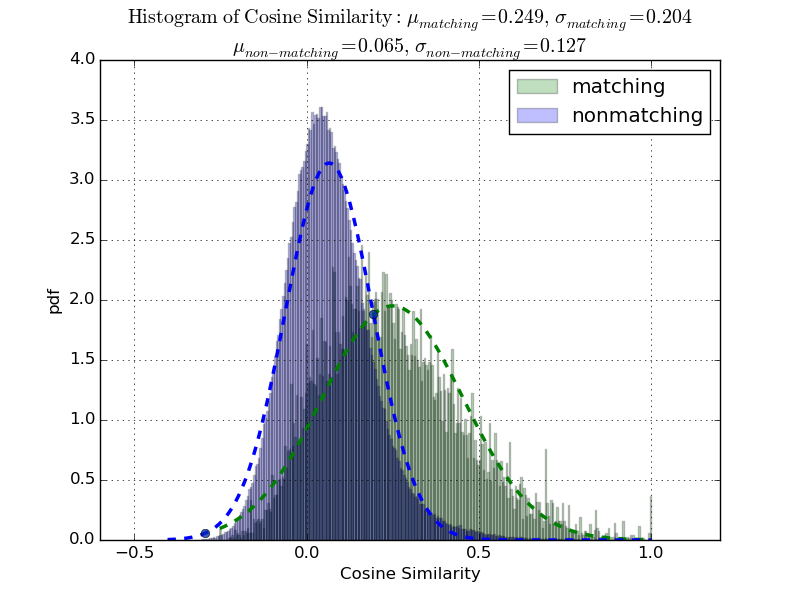
\includegraphics[scale=.40]{match-dist.png} 
\caption{Distribution of nugget similarity for matching and non-matching 
updates.\fdcomment{possible to output this as a vector graphic (pdf pref).  it will scale better.}}
\end{figure}
\subsubsection{Effect of Salience Models}

In order to assess the effectiveness of the salience predictions on update
selection, we perform a baseline (AP-base) run using affinity propagation 
clustering
with uniform preference, i.e. all preferences are equal to the median sentence
similarity. This run is compared to our full system (AP-sal), using each
sentence's salience prediction as its preference. 

We are also interested
in the effect of directly incorporating salience in the clustering algorithm.
A third run (HAC) is performed using hierarchical agglomerative 
clustering; we produce flattened clusters by setting a maximum cluster 
distance threshold. The sentence with the highest predicted salience from each
 cluster is selected as an update. 
The distance threshold was tuned using grid search. By comparing
HAV with AP-base we can empirically assess the trade off between preference
and neighbor similarity that affinity propagation is making.

\subsubsection{Feature Ablation}

We remove each feature group and train models models on these small faller 
feature susbstets. All other parameters are the same as in our full system 
(AP-sal).



